\documentclass[a4paper,12pt, leqno]{report}
\usepackage{amsmath,amsthm,amssymb,enumitem, cclicenses, hyperref,amsfonts,tikz-cd,mathrsfs, tikz}
\usetikzlibrary{matrix, calc, arrows}
\setlength{\parindent}{0cm}
\setlength{\parskip}{6pt}
\tikzset{
	curvedlink/.style={
		to path={
			let \p1=(\tikztostart.east), \p2=(\tikztotarget.west),
			\n1= {abs(\y2-\y1)/4} in
			(\p1) arc(90:-90:\n1) -- ([yshift=2*\n1]\p2) arc (90:270:\n1)
		},
	}
}
\newcommand{\homo}{\mathrm{Hom}}
\newcommand{\Q}{\mathbb{Q}}
\newcommand{\Z}{\mathbb{Z}}
\newcommand{\im}{\mathrm{im}\,}
\newcommand{\id}{\mathrm{id}}
\newcommand{\ind}{\mathrm{Ind}_G}
\DeclareMathOperator{\coker}{coker}

\newtheoremstyle{defprop} % name
{\topsep}                    % Space above
{\topsep}                    % Space below
{\mdseries}                  % Body font
{}                           % Indent amount
{\bfseries}                   % Theorem head font
{.}                          % Punctuation after theorem head
{.5em}                       % Space after theorem head
{}  % Theorem head spec (can be left empty, meaning ‘normal’)
 
\newtheoremstyle{dem} % name
{\topsep}                    % Space above
{\topsep}                    % Space below
{\mdseries}                  % Body font
{}                           % Indent amount
{\itshape}                   % Theorem head font
{.}                          % Punctuation after theorem head
{.5em}                       % Space after theorem head
{}  % Theorem head spec (can be left empty, meaning ‘normal’)          

\newtheoremstyle{prop} % name
{\topsep}                    % Space above
{\topsep}                    % Space below
{\itshape}                  % Body font
{}                           % Indent amount
{\bfseries}                   % Theorem head font
{.}                          % Punctuation after theorem head
{.5em}                       % Space after theorem head
{}  % Theorem head spec (can be left empty, meaning ‘normal’)   

\newtheoremstyle{teor} % name
{\topsep}                    % Space above
{\topsep}                    % Space below
{\itshape}                  % Body font
{}                           % Indent amount
{\bfseries}                   % Theorem head font
{.}                          % Punctuation after theorem head
{.5em}                       % Space after theorem head
{}  % Theorem head spec (can be left empty, meaning ‘normal’)               

\theoremstyle{defprop}
\newtheorem{defprop}{Definición/Proposición}
\newtheorem{definicion}{Definición}
\newtheorem*{ejemplo}{Ejemplo}

\theoremstyle{prop}
\newtheorem{prop}{Proposición}

\theoremstyle{teor}
\newtheorem{teor}{Teorema}

\theoremstyle{dem}
\newtheorem*{dem}{Demostración}

%Flechas
\newcommand\rightthreearrow{%
	\mathrel{\vcenter{\mathsurround0pt
			\ialign{##\crcr
				\noalign{\nointerlineskip}$\rightarrow$\crcr
				\noalign{\nointerlineskip}$\rightarrow$\crcr
				\noalign{\nointerlineskip}$\rightarrow$\crcr
			}%
	}}%
}

\newcommand\rightfourarrow{%
	\mathrel{\vcenter{\mathsurround0pt
			\ialign{##\crcr
				\noalign{\nointerlineskip}$\rightarrow$\crcr
				\noalign{\nointerlineskip}$\rightarrow$\crcr
				\noalign{\nointerlineskip}$\rightarrow$\crcr
				\noalign{\nointerlineskip}$\rightarrow$\crcr
			}%
	}}%
}



% Title Page
\title{Cohomología de cuerpos de números}
\author{Daniel Martínez Marqués}


\begin{document}
\chapter*{Cohomología de grupos profinitos}

Estas son las notas correspondientes al seminario del mismo nombre celebrado en la Universidad Autónoma de Madrid durante el curso 2019/2020. Están basadas en el libro \textit{Cohomology of Number Fields} de J. Neukirch, A. Schmidt y K. Wingberg, el cual puede consultarse para usos no comerciales en \url{https://www.mathi.uni-heidelberg.de/~schmidt/NSW2e/}. 
\begin{center}
\cc \ccby \ccnc
\end{center}

\section*{Background check}
Sea $R$ un anillo conmutativo con unidad.
\begin{definicion}
	Un $R$-módulo por la izquierda es un grupo abeliano $M$ con un homomorfismo de anillos $\omega: R \rightarrow \mathrm{End}(M,M)$. Escribimos $ra$ para denotar $\omega(r)(a)$.
\end{definicion}
\begin{definicion} (Límite inverso)
	Sea $(I,\leq)$ un conjunto parcialmente ordenado y dirigido. Sea $\{A_i\}_{i \in I}$ una familia de objetos en una categoría $\mathcal{A}$ y sea $\{f_{ij}\}_{i\leq j}$ una familia de morfismos que verifican $f_{ij}\in \mathrm{Mor}(A_j,A_i)$, $f_{ii}=\id_{A_i}$ y $f_{ik}=f_{ij}\circ f_{jk}$ para $i\leq j \leq k$. A $((A_i)_{i \in I}, (f_{ij})_{i\leq j})$ le llamamos un sistema inverso.
	
	Un límite inverso del sistema inverso es un objeto $A$ en la misma categoría con morfismos $p_i: A \rightarrow A_i$ (llamados proyecciones) tal que $p_i = f_{ij}\circ p_j$ para todo $i\leq j$. Este objeto verifica que cualquier dado cualquier otro par $(B,q_i)$ existe un único morfismo $\phi: A \rightarrow B$ tal que el famoso diagrama conmuta. 
\end{definicion}

\begin{definicion} (Límite directo)
	Sea $(I,\leq)$ un conjunto parcialmente ordenado y dirigido. Sea $\{A_i\}_{i \in I}$ una familia de objetos en una categoría $\mathcal{A}$ y sea $\{f_{ij}\}_{i\leq j}$ una familia de morfismos que verifican $f_{ij}\in \mathrm{Mor}(A_i,A_j)$, $f_{ii}=\id_{A_i}$ y $f_{ik}=f_{jk}\circ f_{ij}$ para $i\leq j \leq k$. A $((A_i)_{i \in I}, (f_{ij})_{i\leq j})$ le llamamos un sistema directo.
	
	Un target es un par $(X,(\phi_i)_{i\in I})$ donde $X$ es un objeto en la categoría y los $\phi: X_i \rightarrow X$ verifican $\phi_i = \phi_j \circ f_{ij}$ para $i \leq j$. Un límite directo es un target tal que para cualquier otro $(Y,(\psi_i)_{i\in I})$ hay un único morfismo $u:X \rightarrow Y$ tal que el famoso diagrama conmuta. 
	

\end{definicion}
En ambas definiciones, si $X'$ es otro objeto que verifica lo mismo existen isomorfismos que conmutan con los morfismos descritos. 
\begin{prop}
La categoría de $R$-módulos (y en general las cosas algebraicas) tienen límites inversos. 
\end{prop}
\begin{dem}
	Afirmo que $L=\{(a_i) \in \prod A_i:a_i=f_{ij}(a_j),i\leq j\}$ con las proyecciones obvias es el límite inverso. Que satisface $p_i=f_{ij}\circ p_j$ está claro por definición. 
	
	Supongamos que $(L',(q_i))$ verifica lo mismo. Tenemos que demostrar que existe un único $\phi: L' \rightarrow L$ tal que $q_i=p_i \circ \phi$. Por cómo está definido $L$ (producto) está claro cómo construir $\phi$ que verifica eso, lo que tenemos que demostrar es que $\im \phi \subseteq L$ y que es único. 
	
	Observamos que $p_i(\phi(l'))=q_i(l')=f_{ij}(q_j(l'))=f_{ij}(p_j(\phi(l')))$ luego $\phi(l')\in P$. Ahora supongamos que existe un $\psi$ tal que  $i \circ \phi = i \circ \psi$ tiene los mismos valores al precomponerlo con los $p_i$ (luego son  iguales en el el producto). Como $i$ es inyectivo $j=k$.
\end{dem}
\section*{Grupos profinitos}

Prerrequisitos:

\begin{itemize}
	\item Topología y álgebra al nivel de tercero del grado.
	\item Saber qué es un límite inverso y el producto tensorial.
\end{itemize}

Estos grupos topológicos aparecen al considerar los grupos de Galois de extensiones infinitas de cuerpos.
\begin{defprop} \label{prof1}
	Decimos que un espacio topológico Hausdorff $T$ es profinito si satisface alguna de las tres siguientes propiedades equivalentes:
	\begin{enumerate}[label=\roman*)]
		\item $T$ es el límite inverso de espacios finitos discretos.
		\item $T$ es compacto y todo punto tiene una base de entornos formada por conjuntos clopen. 
		\item $T$ es compacto y totalmente desconectado.
	\end{enumerate}
\end{defprop}
\begin{dem}
	
i) $\Rightarrow$ ii): el límite inverso de espacios compactos es compacto. Esto se debe a que $\varprojlim X_i$ es un subespacio cerrado de $\prod_{i \in I}X_i$, que a su vez es compacto por el teorema de Tychonoff. 

Recordemos que la topología del límite inverso es la más fina tal que las proyecciones $\pi_i: T \rightarrow X_i$ son continuas, luego en cualquier punto podemos encontrar una base de entornos de la forma $\{\pi_i^{-1}(U)\}$ donde $U\subset X_i$ es clopen. 

ii) $\Rightarrow$ iii): sea $C_t$ la componente conexa de $t \in T$. Como $T$ es compacto y Hausdorff, $C_t$ es la intersección de todos los conjuntos clopen que contienen a $t$; i.e. $C_t=\{t\}$.

iii) $\Rightarrow$ i): sea $I$ el conjunto de relaciones de equivalencia $R$ tal que al cocientar $T/R$ es finito y discreto en la topología del cociente. $I$ está parcialmente ordenado por inclusión y todo par $R_1,R_2$ tiene cota superior $R_1 \cap R_2$, luego $I$ es dirigido. Afirmo que $\phi: T \rightarrow \ \varprojlim T/R$ es un homeomorfismo. 

Demostramos primero que $\phi$ es sobreyectivo: sea $\{t_R\}_{R \in I} \in  \varprojlim T/R $. Nótese que los conjuntos $(p_R \circ \phi)^{-1}(t_R)$ son no vacíos y compactos (son preimagenes de un compacto y $T$, $T/R$ son compacto y Hausdorff respectivamente). Al ser $I$ dirigido esto implica que intersecciones finitas de estos conjuntos tambien son no vacías y por compacidad obtenemos que $\phi^{-1}(\{t_R\}_{R\in I})= \cap_{R \in I}(p_R \circ \phi)^{-1}(t_R)$ también es no vacío. (Un espacio es compacto si y solo si cualquier colección de subconjuntos cerrados con la propiedad de intersección finita tiene interseccion no vacía).

Para ver que $\phi$ es inyectiva es suficiente demostrar que para $t,s \in T$ distintos, existe $R \in I$ tal que $(t,s)\notin R$. Como $T$ es totalmente desconectado $s\notin C_t$. Por la caracterización nombrada anteriormente, existe un subconjunto clopen $U \subseteq T$ tal que $t\in U$, $s \notin U$ y definimos una relación de equivalencia $R$: $(x,y)\in R$ si y solo si $x$ e $y$ están ambos en $U$ o $U^c$. $R$ cumple la condición requerida luego $\phi$ es una biyección entre espacios compactos, es decir, un homeomorfismo. \qed
\end{dem}
\begin{defprop}
	Decimos que un grupo topológico Hausdorff $G$ es un grupo profinito si satisface alguna de las siguiente condiciones equivalentes:
	\begin{enumerate}[label=\roman*)]
		\item $G$ es el límite inverso topológico de grupos finitos discretos.
		\item $G$ es compacto y el elemento neutro tiene una base de entornos formada por subgrupos normales clopen. 
		\item $G$ es compacto y totalmente desconectado.
	\end{enumerate}
\end{defprop}
\begin{dem}
	i) $\Rightarrow$ iii): el límite inverso de espacios compactos y totalmente desconectados es a su vez compacto y totalmente desconectado. 
	
	ii) $\Rightarrow$ i): sea $\{N_e\}$ el conjunto de entornos de $e \in G$ que son subgrupos normales abiertos. Afirmo que el homomorfismo canónico $\phi: G \rightarrow \varprojlim_U G/U$ es un isomorfismo. Es fácil ver que es inyectiva: si no lo fuese, existiría un $g \in G$ tal que $g \in N_e$ para todo entorno de la colección, lo cual contradice que $G$ es Hausdorff. 
	
	Demostramos ahora que es sobreyectiva. Sea $x=\{x_U\}_U\in \varprojlim_U G/U$. Sea $\phi_U:G \rightarrow G/U$ la proyección canónica. Tenemos una igualdad:
	\begin{equation*}
	\phi^{-1}(x)=\bigcap\limits_{U} \phi^{-1}_U(x_U).
	\end{equation*}
	Nótese que la intersección de la derecha es no vacía utilizando el mismo argumento que en la demostración de \ref{prof1}. Por lo tanto $\phi$ es biyectiva y de hecho también es una aplicación abierta, luego es un homeomorfismo. Por otra parte, es claro que para cada $U$, $G/U$ es compacto y discreto, luego es finito. 
	
	iii) $\Rightarrow$ ii): el espacio topológico que subyace a $G$ es profinito por \ref{prof1}, luego todo punto tiene una base de entornos formada por conjuntos clopen. Nótese que un subconjunto abierto es automáticamente cerrado porque es el complementario de la unión de sus clases laterales no triviales, que son abiertas. Sea $U$ un entorno clopen de $e\in G$, definimos:
	\begin{center}
		$V:=\{v \in U|Uv\subseteq U\}$ y $H:=\{h \in V |h^{-1}\in V\}$.
	\end{center}
Afirmo que $H \subseteq U$ is un subgrupo clopen en $G$. Primero demostraremos que $V$ es abierto: sea $v\in V$. Por definición $uv \in V$ para todo $u\in U$, luego existen entornos $U_u$ de $u$ y $V_u$ de $v$ tal que $U_u V_u \subseteq U$. Los conjuntos abiertos $\{U_u\}$ cubren el espacio compacto $U$, luego existe un subrecubrimiento finito $U_{u_1},...,U_{u_n}$. 

Sea $V_v := V_{u_1}\cap \cdots \cap V_{u_n}$. $V_v$ es un entorno abierto de $v$ contenido en $V$, luego $V$ es abierto y $H:= V \cap V^{-1}$ porque invertir es un homeomorfismo. Solo falta demostrar que $H$ es un subgrupo. Es claro que $e \in H$ y que $H^{-1}=H$, luego nos queda comprobar que si $x,y \in H$ entonces $xy \in H$. Nótese pprimero que $Uxy \subseteq Uy \subset U$, por lo que $xy \in V$. Con el mismo razonamiento uno obtiene que $(xy)^{-1}\in V$, luego $xy \in H$. Es decir, $H$ es un subgrupo abierto de $G$ contenido en $U$. En particular, $H$ tiene índice finito en $G$ y solo hay un número finito de conjugados de $H$. La intersección de estos conjugados es un subgrupo clopen normal de $G$ contenido en $U$. \qed
\end{dem}

De ahora en adelante, todos los homomorfismos entre grupos profinitos serán continuos salvo que se indique lo contrario. De la misma manera, todos los subgrupos serán cerrados. Como ya se dijo anteriormente, los subgrupos abiertos son inmediatamente cerrados y por compacidad, es sencillo ver que los subgrupos cerrados son abiertos si y solo si tienen índice finito. 

Si $H$ es un subgrupo de un grupo profinito $G$, el conjunto $G/H$ de clases laterales es un espacio profinito con la topología del cociente. Si $H$ es un subgrupo normal, $G/H$ es un grupo profinito en la manera natural de cocientar. En general, toda la teoría de grupos tiene un análogo para el caso de grupos topológicos profinitos. A continuación veremos ejemplos de este paralelismo.
\begin{definicion}
	Un \textbf{número supernatural} es un producto formal $\prod\limits_{p}p^{n_p}$, donde $p$ recorre los primos y $n_p$ son enteros no negativos o $\infty$.
\end{definicion}
Podemos multiplicar números supernaturales sumando los exponentes de la manera natural. También existen las nociones de máximo común divisor y mínimo común múltiplo. 
\begin{definicion}
	Sean $G$ un grupo profinito y $A$ un  grupo abeliano con torsión. 
	\begin{enumerate}[label=\roman*)]
		\item El \textbf{índice} de un subgrupo cerrado $H$ de $G$ es el número supernatural:
		\begin{equation*}
		(G:H)=\mathrm{m.c.m.}\{(G/U:H/H\cap U)\},
		\end{equation*}
		donde $U$ recorre los subgrupos normales abiertos de $G$. 
		\item  El \textbf{orden} de $G$ se define como $\#G=(G:1)=\mathrm{m.c.m.}\{\#(G/U)\}_U$. 
		\item El \textbf{orden} de $A$ se define como $\#A=\mathrm{m.c.m.} \{\#B\}$, donde $B\leq A$ recorre los subgrupos finitos de $A$.
	\end{enumerate}
\end{definicion}
Dada una cadena de subgrupos cerrados $N\leq H \leq G$ el índice se comporta de manera multiplicativa, es decir:
\begin{equation*}
(G:N)=(G:H)(H:N)
\end{equation*}
Observamos que el orden de un grupo abeliano con torsión $A$ coincide con el orden del grupo profinito $ \homo (A, \Q / \Z)$.
\begin{definicion}
	Sea $G$ un grupo profinito. Un \textbf{$G$-módulo abstracto} $M$ es un grupo abeliano $M$ con una acción:
	\begin{equation*}
	G \times M \rightarrow M, (g,m)\mapsto g(m)
	\end{equation*}
	tal que $1(m)=m$, $(gh)(m)=g(h(m))$ y $g(m+n)=g(m)+g(n)$ para todo $g,h \in G$ y $m,n \in M$.
	
		Un \textbf{$G$-módulo topológico} $M$ es un grupo topológico abeliano y Hausdorff con la estructura de un $G$-módulo abstracto tal que la acción $G \times M \rightarrow M$ es continua. 
\end{definicion}
\begin{prop}
Sean $G$ un grupo profinito y $M$ un $G$-módulo abstracto. Las siguientes condiciones son equivalentes:
\begin{enumerate}[label= \roman*)]
	\item $M$ es un $G$-módulo (topológico) discreto; es decir, la acción $G \times M \rightarrow M$ es continua con la topología discreta en $M$.
	\item Para todo $m \in M$ el estabilizador $G_m:=\{g \in G|g(m)=m\}$ es abierto.
	\item $M=\bigcup M^U$, donde $U$ recorre los subgrupos abiertos de $G$. 
\end{enumerate}
\end{prop}
\begin{dem}
	i) $\Rightarrow$ ii): si restringimos la acción a $G \times \{m\}$, tenemos que la preimagen de $m$ es $G_m$. Al ser la acción continua por hipótesis, $G_m$ es abierto. 
	
	ii) $\Rightarrow$ iii): trivial porque $m \in M^{G_m}$ y los $G_m$ son abiertos por hipótesis.
	
	iii) $\Rightarrow$ i): sea $(g,m)\in G \times M$. Sabemos que existe un subgrupo abierto $U$ tal que $m \in M^U$, luego $gU \times \{m\}$ es un entorno abierto de $(g,m)$ que va a parar a $g(m)$. Luego la acción es continua. \qed
\end{dem}
En lo que a estas notas respecta nos centraremos en $G$-módulos topológicos discretos y normalmente omitiremos tanto la terminología \textit{abstracto} como \textit{topológico} cuando nos refitamos a estos.
\paragraph*{Ejemplos de operaciones con $G$-módulos:}
\begin{enumerate}
	\item Dada una familia $(A_i)_{i\in I}$ de $G$-módulos discretos, la suma directa $\bigoplus_{i \in I}A_i$ es también un $G$-módulo discreto donde $G$ actúa en cada coordenada: $g((a_i)_{i \in I})=(g(a_i))_{i \in I}$. 
	
	Esto no es cierto en general para el producto directo. 
	
	\item El producto tensorial $A \otimes B$ sobre $\mathbb{Z}$ de dos $G$-módulos discretos es de nuevo un $G$-módulo discreto con la acción diagonal de $G$: $g(a \otimes b)=g(a) \otimes g(b)$.
	\item Al conjunto $\homo_{\Z}(A,B)$ se le puede dar la estructura de $G$-módulo abstracto definiendo la acción $g(\phi)(a)=g(\phi(g^{-1}(a)))$. 
	
	Si $A=A^U$ para algún subgrupo abierto $U\leq G$, entonces $\homo (A,B)$ es un $G$-módulo discreto. Esto ocurre por ejemplo cuando $G$ es finito o si $A$ es finitamente generado como $\Z$-módulo. 
	\item Los grupos $\Z, \Q, \Z/n\Z$ y $\mathbb{F}_q$ se pueden ver como $G$-módulos discretos con acción trivial. 
\end{enumerate}	
Hasta ahora, todos los grupos que hemos considerado han sido compactos y totalmente desconectado. 


\section*{Grupos de cohomología}
Sea $G$ un grupo profinito, en esta sección todos los $G$-modulos serán discretos. Consideremos el diagrama:
\begin{equation*}
	\cdots \rightfourarrow G \times G \times G \rightthreearrow G \times G \rightrightarrows G,
\end{equation*}
donde las flechas representan las proyecciones $d_i:G^{n+1}\rightarrow G_n$ para $i=0,1,...,n$ dadas por:
\begin{equation*}
d_i(\sigma_0,...,\sigma_n)=(\sigma_0,...,\hat{\sigma}_i,...,\sigma_n)
\end{equation*}
donde $\hat{\sigma_i}$ significa que omitimos ese término. Dado un $G$-módulo $A$ definimos el grupo abeliano:
\begin{equation*}
X^n(G,A)=\mathrm{Map}(G^{n+1},A)
\end{equation*}
de funciones continuas $x: G^{n+1}\rightarrow A$. $X^n$ tiene estructura natural de $G$-módulo con la acción:
\begin{equation*}
(\sigma x)(\sigma_0,...,\sigma_n)=\sigma x(\sigma^{-1}\sigma_0,...,\sigma^{-1}\sigma_n).
\end{equation*}
Obsérvese que la proyección $d_i$ induce un $G$-homomorfismo $d_i^*:X^{n-1}\rightarrow X^n$, y podemos formar la suma:
\begin{equation*}
\partial^n=\sum_{i=0}^{n}(-1)^i d_i^*.
\end{equation*}
Explícitamente, para $x \in X^{n-1}, \partial^n x$ es la función:
\begin{equation*}
(\partial^n x)(\sigma_0,...,\sigma_n)=\sum_{i=0}^{n}(-1)^i x(\sigma_0,...,\hat{\sigma_i},...,\sigma_n).
\end{equation*}
Tenemos además otro $G$-homomorfismo $\partial^0: A \rightarrow X^0$ definido como $a \mapsto x$ donde $x$ es la functión constante con valor $a$.
\begin{prop}
	La sucesión:
\begin{center}
	\begin{tikzcd}
	0 \arrow{r}& A \arrow{r}{\partial^0}& X^0 \arrow{r}{\partial^1}& X^1 \arrow{r}{\partial^2}& X^2 \arrow{r}& \cdots
	\end{tikzcd}
\end{center}
es exacta.
\end{prop}
\begin{dem}
	La comprobación de que $\im \partial^i \subseteq \ker \partial^{i+1}$ es directa. Para comprobar que es exacta consideramos las funciones $D^{-1}:X^0 \rightarrow A,D^{-1}x=x(1)$ y para $n\geq 0$:
	\begin{equation*}
	D^n:X^{n+1} \rightarrow X^n,(D^n x)(\sigma_0,...,\sigma_n)=x(1,\sigma_0,...,\sigma_n).
	\end{equation*}
	Los $D^n$ son homomorfismos de grupos abeliano pero no de $G$-módulos. Es fácil comprobar que:
	\begin{equation*}
	D^n \circ \partial^{n+1}+\partial^n\circ D^{n-1} = \id,
	\end{equation*}
	luego si $x \in \ker \partial^{n+1}$ entonces $x=\partial^n(D^{n-1}x)$. Es decir $\ker \partial^{n+1}\subseteq \im \partial^n$. \qed
\end{dem}
\begin{definicion}
	A una sucesión exacta de $G$-módulos:
	\begin{equation*}
	0 \rightarrow  A \rightarrow X^0 \rightarrow X^1 \rightarrow \cdots
	\end{equation*}
	se le llama una \textbf{resolución} de $A$. A ésta en concreto se le denomina la resolución estándar. A una familia $(D^n)_{n\geq 1}$ como la de la demostración anterior se le llama una homotopía. 
\end{definicion}
A continuación vamos a seleccionar los elementos $G$-invariantes de $X^n(G,A)$ y los vamos a denotar $C^n(G,A)=X^n(G,A)^G$. Es decir aquellas funciones $x: G^{n+1}\rightarrow X$ tal que para todo $\sigma \in G$:
\begin{equation*}
x(\sigma \sigma_0,...,\sigma \sigma_n)=\sigma x(\sigma_0,...,\sigma_n).
\end{equation*}
A $C^n$ le llamamos la $n$-cocadenas de $G$ con coeficientes en $A$. Aplicando el functor $A \mapsto A^G$ a toda la resolución estándar obtenemos una secuencia que en general deja de ser exacta:
\begin{center}
	\begin{tikzcd}
	 C^0(G,A) \arrow{r}{\partial^1}& C^1(G,A) \arrow{r}{\partial^2}& C^2(G,A) \arrow{r}& \cdots
	\end{tikzcd}
\end{center}
Sin embargo todavía se verifica que $\partial \partial =0$ y normalmente se le llama el complejo de cocadenas homogéneas de $G$ con coeficientes en $A$.
\begin{definicion}
	Definimos los $n$-cociclos como:
	\begin{equation*}
	Z^n(G,A)=\ker \partial^{n+1}.
	\end{equation*}
	Definimos los $n$-cobordes como:
	\begin{equation*}
	B^n(G,A)= \im \partial^n.
	\end{equation*}
	Obsérvese que la condicion $\partial \partial=0$ garantiza que $B^n(G,A)\subseteq Z^n(G,A)$.
	
	Para $n\geq 0$ definimos \textbf{grupo de cohomología} $n$-dimensional de $G$ con coeficientes en $A$:
	\begin{equation*}
	H^n(G,A)=Z^n(G,A)/B^n(G,A).
	\end{equation*}
\end{definicion}
En muchas ocasiones trabajaremos con una versión ligeramente modificada de los grupos de cohomología que reduce el número de variables de las cocadenas. Sea $\mathscr{C}^0(G,A)=A$ y para $n\geq 1$ $\mathscr{C}^n(G,A)$ el grupo abeliano de funciones continuas $y:G^n\rightarrow A$. Tenemos isomorfismos:
\begin{equation*}
C^0(G,A)\rightarrow \mathscr{C}^0(G,A),x(\sigma)\mapsto x(1)
\end{equation*}
y para $n\geq 1$ $C^n \rightarrow \mathscr{C}^n(G,A)$:
\begin{equation*}
x(\sigma_0,...,\sigma_n)\mapsto y(\sigma_1,...,\sigma_n)=x(1,\sigma_1,\sigma_1 \sigma_2,...,\sigma_1...\sigma_n).
\end{equation*}
Obsérvese que el inverso de este isomorfismo viene dado por:
\begin{equation*}
y(\sigma_1,...,\sigma_n)\mapsto x(\sigma_0,...,\sigma_n)=\sigma_0 y(\sigma_0^{-1}\sigma_1,\sigma_1^{-1}\sigma_2,...,\sigma_{n-1}^{-1}\sigma_n).
\end{equation*}
Esto nos permite reescribrir los operadores coborde:
\begin{equation*}
\partial^{n+1}:\mathscr{C}^n(G,A)\rightarrow \mathscr{C}^{n+1}(G,A),
\end{equation*}
dados por:
\begin{align*}
(\partial^1 a)(\sigma)= \sigma a -a & &\text{for } a\in A=\mathscr{C}^0(G,A),\\
(\partial^2 y)(\sigma,\tau)=\sigma y(\tau)-y(\sigma \tau)+y(\sigma) & & \text{for } y\in \mathscr{C}^1(G,A).
\end{align*}
Para el resto:
\begin{align*}
(\partial^{n+1}y)(\sigma_1,...,\sigma_{n+1})&=\sigma_1y(\sigma_2,...,\sigma_{n+1})
+\sum_{i=1}^{n}(-1)^i y(\sigma_1,...,\sigma_{i-1},\sigma_i,\sigma_{i+1},\sigma_{i+2},...,\sigma_{n+1})\\
&+(-1)^{n+1}y(\sigma_1,...,\sigma_n),
\end{align*}
donde $y\in \mathscr{C}^N(G,A)$. Si ahora definimos:
\begin{align*}
\mathscr{L}^n(G,A)&=\ker \partial^{n+1}\\
\mathscr{B}^n(G,A)&=\im \partial^n,
\end{align*}
los isomorfismos $C^n(G,A)\simeq \mathscr{C}^n(G,A)$ inducen isomorfismos:
\begin{equation*}
H^n(G,A)\simeq \mathscr{L}^n(G,A)/\mathscr{B}^n(G,A).
\end{equation*}
A estos/as $n$-cocadenas, $n$-cociclos y $n$-cobordes se les denomina inhomogéneos.
\paragraph*{Interpretando el grupo $H^0(G,A)$:} recordamos que hay un isomorfismo $C^0(G,A)\rightarrow A$ dado por $x\mapsto x(1)$. Según hemos visto arriba, $(\partial^1 a)(\sigma)=\sigma(a)-a$.  Es decir:
\begin{equation*}
H^0(G,A)=\ker \partial^1 A^G.
\end{equation*}
\paragraph*{Interpretando el grupo $H^1(G,A)$:} de nuevo recordamos que los $1$-cociclos inhomogéneos vienen dados por funciones $x: G \rightarrow A$ tal que para todo $\sigma,\tau \in G$:
\begin{equation*}
x(\sigma \tau)=x(\sigma)+\sigma x(\tau).
\end{equation*}
Los $1$-cobordes son las funciones dados por $x(\sigma)=\sigma(a)-a$ para $a\in A$ fijo.  Obsérvese que si $G$ actúa trivialmente, $H^1(G,A)$ es simplement $\homo_{cts}(G,A)$. De manera más general, la motivación para definir $H^1$ viene de considerar una sucesión corta exacta:
\begin{center}
\begin{tikzcd}
0 \arrow{r} & A \arrow{r}{i} & B \arrow{r}{j} & C \arrow{r} & 0. 
\end{tikzcd}
\end{center}
Si tomamos los elementos fijados por $G$, en general un elemento de $C^G$ no puede ser representado por uno de $B^G$ y la sucesión deja de ser exacta por la derecha:
\begin{center}
	\begin{tikzcd}
	0 \arrow{r} & A^G \arrow{r} & B^G \arrow{r} & C^G. 
	\end{tikzcd}
\end{center}
En este caso $H^1$ mide cuánto de lejos está de ser exacta esa sucesión. De hecho, hay un isomorfismo canónico:
\begin{equation*}
\delta: C^G \rightarrow H^1(G,A)
\end{equation*} 
que extiende a una sucesión que exacta:
\begin{center}
	\begin{tikzcd}
	0 \arrow{r} & A^G \arrow{r} & B^G \arrow{r} & C^G \arrow{r}{\delta}& H^1(G,A). 
	\end{tikzcd}
\end{center}
(Durante el seminario, se hará una demostración de \textit{diagram chase}).

Para dar una interpretación aún más concreta introduciremos el concepto de \textit{torsor}. Para poder explotarlo a fondo olvidaremos la hipótesis de que $A$ es abeliano, lo cual nos obliga a hacer algunas modificaciones:
\begin{definicion}
	Un \textbf{$G$-grupo} $A$ es un grupo no necesariamente abeliano con la topología discreta y acción de $G$ continua. La acción de $G$ suele denotarse con $a^{\sigma}$. 
	
	Un \textbf{cociclo} de $G$ con coeficientes en $A$ es una función continua $\sigma \mapsto a(\sigma)$ tal que:
	\begin{equation*}
	a(\sigma \tau)=a(\sigma)a(\tau)^{\sigma}.
	\end{equation*}
	Al conjunto de cociclos lo denominamos $\mathscr{L}^1(G,A)$. Dos cociclos son cohomólogos si existe algún $b\in A$ tal que:
	\begin{equation*}
	a'(\sigma)=b^{-1}a(\sigma) b^{\sigma}.
	\end{equation*}
	Esto es una relación de equivalencia y al cociente le denominamos $H^1(G,A)$ (pointed set).
\end{definicion}

\section*{La sucesión exacta }
A continuación estudiaremos cómo se comporta $H^n$ con respecto a homomorfisms ode $G$-módulos $f:A \rightarrow B$. Este $f$ induce un homomorfismo entre las cocadenas $f: C^n(G,A) \rightarrow C^n(G,B)$ que conmuta con $\delta$, luego también induce un homomorfismo:
\begin{equation*}
f: H^n(G,A)\rightarrow H^n(G,B).
\end{equation*}
\begin{prop}
	\textit{Snake Lemma:}
	
	
	\begin{center}
		
		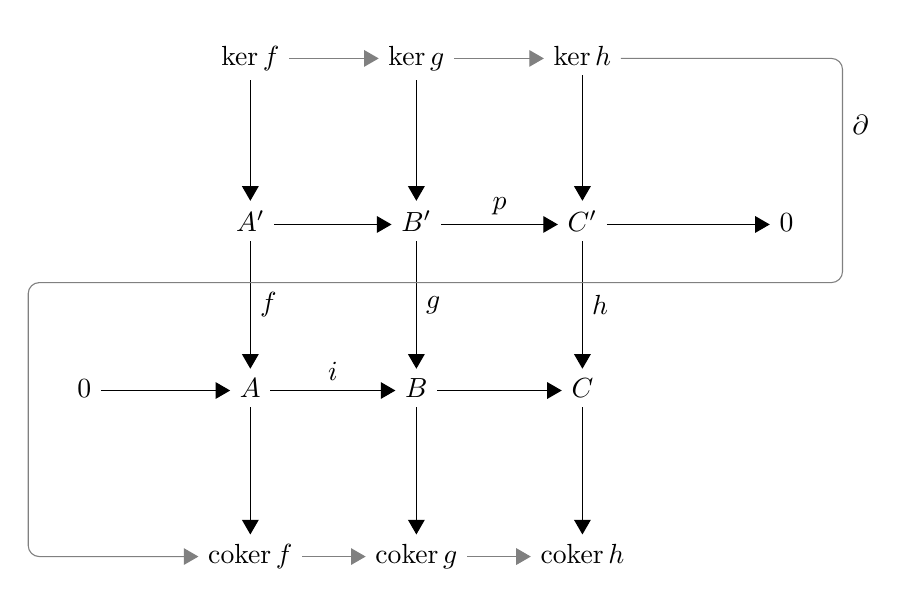
\begin{tikzpicture}[>=triangle 60]
		
		\matrix[matrix of math nodes,column sep={60pt,between origins},row
		sep={60pt,between origins},nodes={asymmetrical rectangle}] (s)
		{
			&|[name=ka]| \ker f &|[name=kb]| \ker g &|[name=kc]| \ker h \\
			%
			&|[name=A]| A' &|[name=B]| B' &|[name=C]| C' &|[name=01]| 0 \\
			%
			|[name=02]| 0 &|[name=A']| A &|[name=B']| B &|[name=C']| C \\
			%
			&|[name=ca]| \coker f &|[name=cb]| \coker g &|[name=cc]| \coker h \\
		};
		\draw[->] (ka) edge (A)
		(kb) edge (B)
		(kc) edge (C)
		(A) edge (B)
		(B) edge node[auto] {\(p\)} (C)
		(C) edge (01)
		(A) edge node[auto] {\(f\)} (A')
		(B) edge node[auto] {\(g\)} (B')
		(C) edge node[auto] {\(h\)} (C')
		(02) edge (A')
		(A') edge node[auto] {\(i\)} (B')
		(B') edge (C')
		(A') edge (ca)
		(B') edge (cb)
		(C') edge (cc)
		;
		\draw[->,gray] (ka) edge (kb)
		(kb) edge (kc)
		(ca) edge (cb)
		(cb) edge (cc)
		;
		\draw[->,gray,rounded corners] (kc) -| node[auto,text=black,pos=.7]
		{\(\partial\)} ($(01.east)+(.5,0)$) |- ($(B)!.35!(B')$) -|
		($(02.west)+(-.5,0)$) |- (ca);
		\end{tikzpicture}
		
	\end{center}
\end{prop}

El hecho crucial que podemos demostrar con este lema es que dada una sucesión exacta:
\begin{equation*}
0 \rightarrow A \rightarrow B\rightarrow C \rightarrow 0
\end{equation*}
existe un homomorfismo canónico para todo $n \geq 0$:
\begin{equation*}
\delta: H^n(G,C)\rightarrow H^{n+1}(G,A)
\end{equation*}
que nos da la siguiente sucesión exacta: 
\begin{center}
	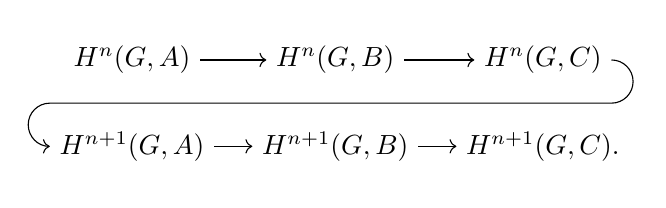
\begin{tikzpicture}
	\centering
	\matrix[matrix of nodes,ampersand replacement=\&, column sep=0.5cm, row sep=0.5cm](m)
	{
		$H^n(G,A)$ \& $H^n(G,B)$ \& $H^n(G,C)$ \\
	 $H^{n+1}(G,A)$ \& $H^{n+1}(G,B)$ \& $H^{n+1}(G,C).$ \\
	};
	\draw[->]
	(m-1-1) edge (m-1-2)
	(m-1-2) edge  (m-1-3)
	(m-1-3)  edge[curvedlink] node {$\partial$}(m-2-1) 
	(m-2-1) edge (m-2-2)
	(m-2-2) edge (m-2-3)
	;
	\end{tikzpicture}
\end{center}
\end{document}          